\providecommand{\main}{../../..}
\documentclass[\main/main.tex]{subfiles}
\begin{document}

\subsection{Esercizio 5}
Si determini la soluzione ottima con la funzione di utilità $u = f_1 - 9f_2^2$ del seguente problema di programmazione a due obbiettivi:

\begin{figure}
  \begin{align*}
    \max f_1 = 9x_1^2 + 4x_2^2 - 18x_1 - 16x_2 \\
    \max f_2 = -x_1                            \\
    3x_1 + x_2  & \leq 6                       \\
    3x_1 + 2x_2 & \leq 9                       \\
    x_2         & \geq 0
  \end{align*}
  \caption{Esercizio 5}
\end{figure}

\subsection{Soluzione esercizio 5}
\subsubsection*{Costruisco funzione obbiettivo composta}
\begin{align*}
  f^*(\bmx) & = 9x_1^2 + 4x_2^2 - 18x_1 - 16x_2 - 9(-x_1)^2 \\
            & = 4x_2^2 - 18x_1 - 16x_2
\end{align*}
\subsubsection*{Risolvo il problema}
\begin{align*}
  \max f^* = 4x_2^2 - 18x_1 - 16x_2 \\
  3x_1 + x_2  & \leq 6              \\
  3x_1 + 2x_2 & \leq 9              \\
  x_2         & \geq 0
\end{align*}

Il problema non è vincolato, per cui la soluzione ottima si ha per $x_1 = \infty$.

\subsubsection*{Verifico la soluzione}

\begin{figure}
  \begin{subfigure}{0.45\textwidth}
    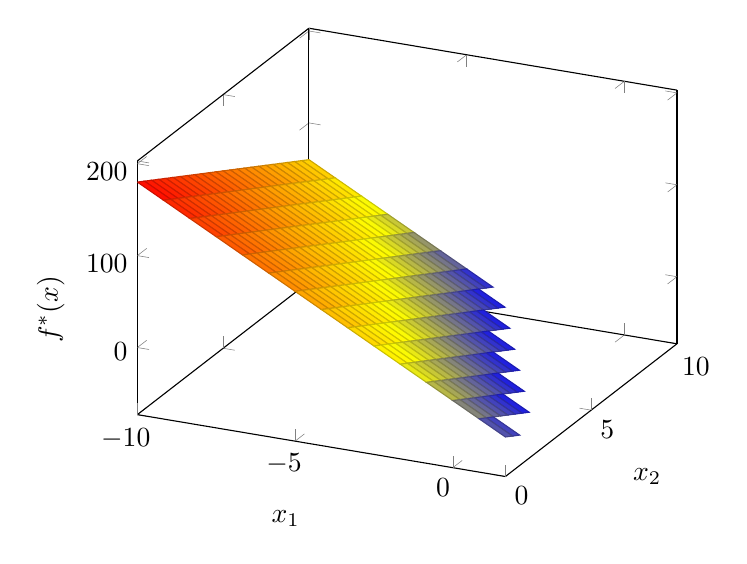
\begin{tikzpicture}
      \begin{axis}[
          xlabel=$x_1$,
          ylabel=$x_2$,
          zlabel=$f^*(x)$,
          domain=-10:10,
          y domain=0:10
        ]
        \addplot3[surf, unbounded coords=jump]
        {3*x + y <= 6 && 3*x + 2*y <= 9? 4*y -18*x-16*y: NaN};
      \end{axis}
    \end{tikzpicture}
    \caption{La funzione $f^*(x)$}
  \end{subfigure}
  ~
  \begin{subfigure}{0.45\textwidth}
    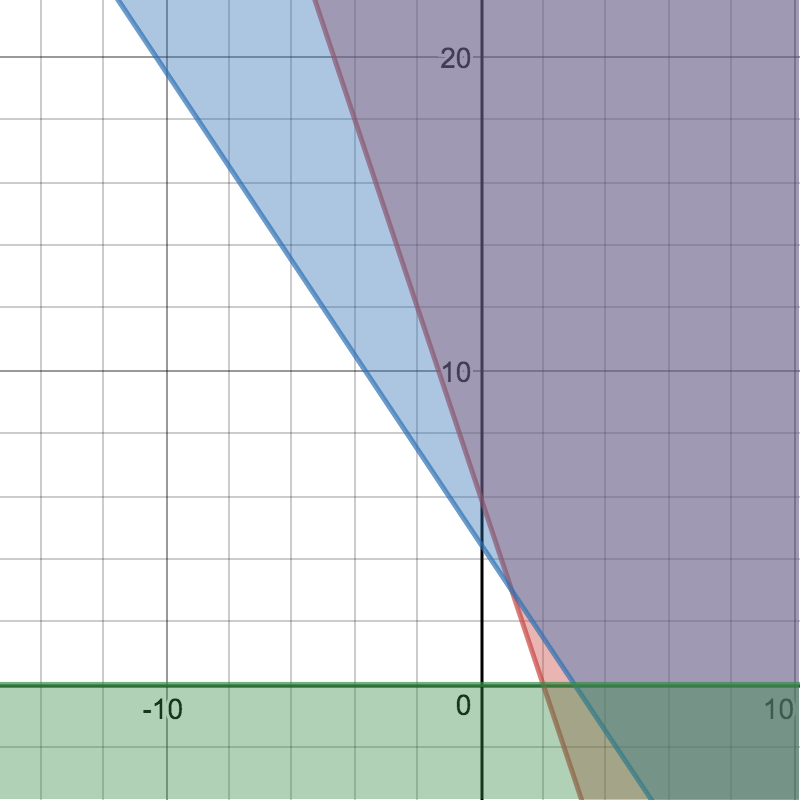
\includegraphics[width=0.8\textwidth]{es5-maut}
    \caption{Dominio della funzione $f^*(x)$}
  \end{subfigure}
\end{figure}

Si conferma che il problema non è vincolato.

\end{document}